\chapter{Autoencoder Network}
\label{ch:autoencoder_network}
Most approaches in style transfer work on the features of an image taken from an encoder network. These features are reconstructed to the image space with a decoder network. Architectures $\Theta = (\phi, \phi^{-1})$ using an encoder $\phi$ and a decoder $\phi^{-1}$ that map their input to its identity via an intermediate representation are called autoencoder networks. 
\begin{align}
\Theta(\mathbf{x})= (\phi^{-1} \circ \phi)(\mathbf{x}) = \mathbf{x}', \quad \mathbf{x} = \mathbf{x}'
\end{align}
This work presents a learned autoencoder network that works with images. At first, the architecture is shown. Further on, different losses are introduced that are used in training. The chapter concludes with experiments.

\section{Architecture}
Figure \ref{fig:autoencoder_network_schematic} shows the whole autoencoder architecture consisting of an encoder and a decoder network.
% figure
\begin{figure}[!ht]
	\centering
  	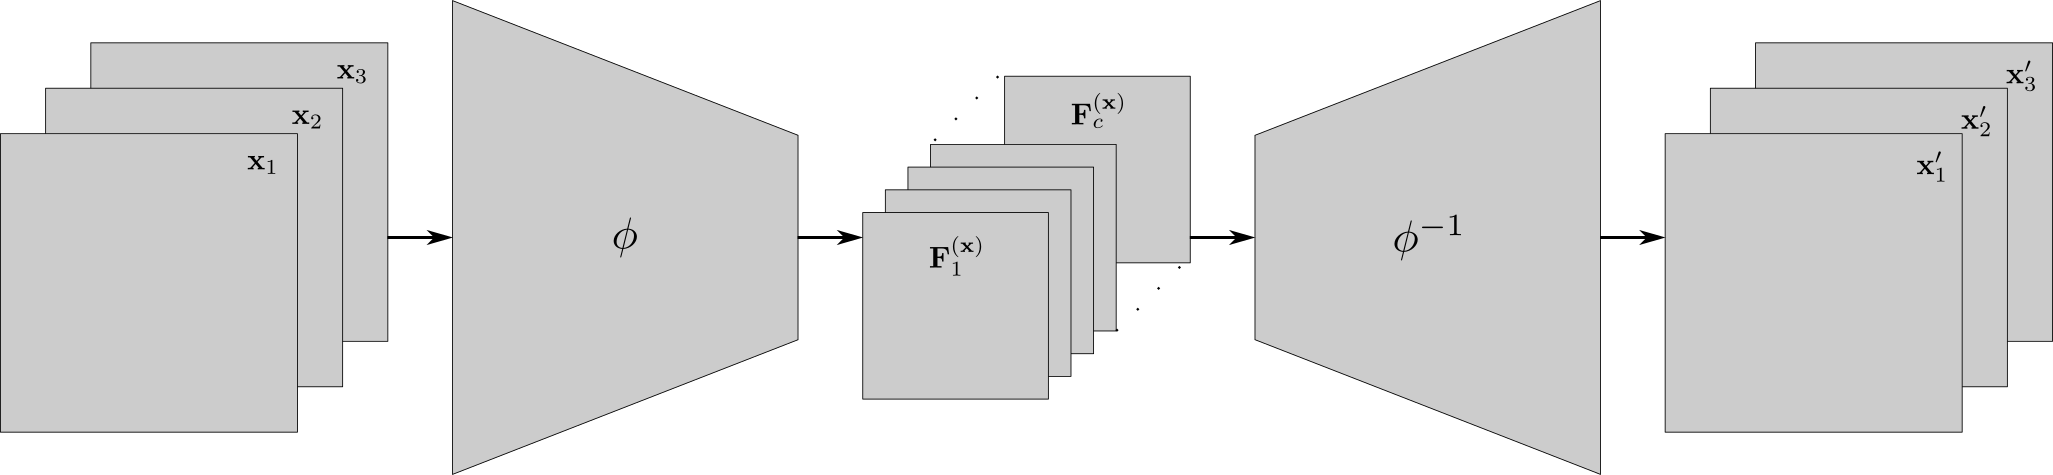
\includegraphics[width=\textwidth]{EncoderDecoder}
	\caption{Autoencoder network.}
	\label{fig:autoencoder_network_schematic}
\end{figure}

\subsection{Encoder}
\label{sec:encoder}
An encoder network is an ANN that learns a representation for a set of data. The aim of encoding data is to reduce its dimensionality and to ignore noise in the input. If one wants to manipulate the given data, encoding can produce representations that make it easier to change the data in a specific way.

In this work, encoding images is done for two main reasons:
\begin{enumerate}
\item
The reduction of dimensionality in the encoding procedure yields feature maps that are easier to manipulate than the original image.

\item
The obtained feature maps represent different characteristics of an input image. An example could be a feature map that detects a certain kind of brushstrokes. Images with this kind of characteristic will produce a high activation in this feature map.
\end{enumerate}

In this work, a pre-trained VGG-19 is used up to the layer \texttt{relu\_4\_1} as an encoder network. 
Figure \ref{fig:encoder_network_layers} shows the encoder network broken down to its layers. Since only convolutional layers are used, input images can have arbitrary sizes.
% figure
\begin{figure}[!ht]
	\centering
  	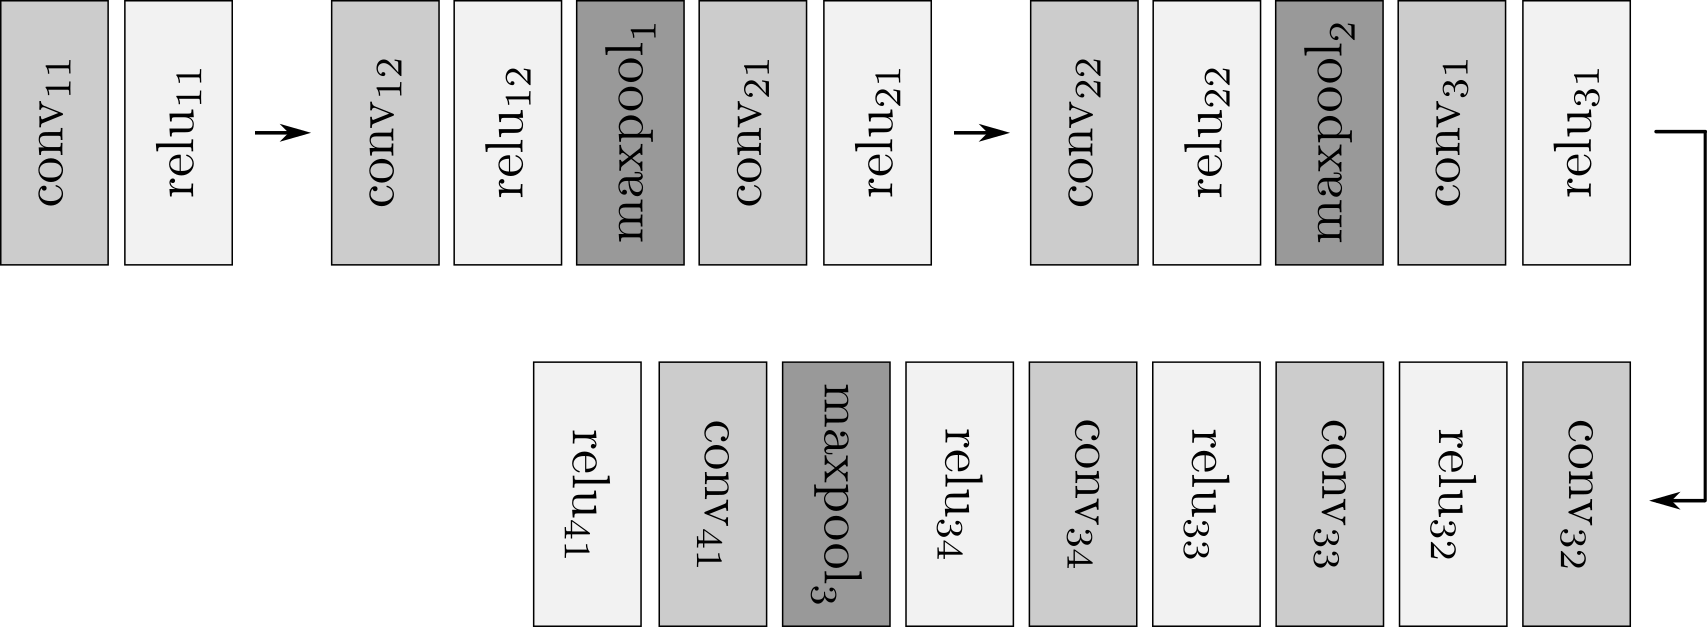
\includegraphics[width=0.65\textwidth]{Encoder_layers}
	\caption{Encoder network broken down to its layers.}
	\label{fig:encoder_network_layers}
\end{figure}

An image $\mathbf{x}$ is encoded by passing it through the encoder network. The activations of each layer $l$ in the forward-pass provide the respective feature space. Let the features at layer $l$ of image $\mathbf{x}$ be referred to as matrix of feature maps.
\begin{align*}
{}_l
\mathbf{F}^{(\mathbf{x})} 
\in 
\mathbb{R}^{c_l \times (h_l \cdot w_l)}
\end{align*}
The features consist of $c_l$ feature maps, each with height $h_l$ and width $w_l$. For ease of readability each feature map is described vectorized by a column vector, where 
\begin{align*}
{}_l
\mathbf{F}^{(\mathbf{x})}_{ij}
\in 
\mathbb{R}^{(h_l \cdot w_l)}
\end{align*}
is the $j$-th entry of the $i$-th feature map at layer $l$. If the layer index $l$ is not specified, the feature response at layer \texttt{relu\_4\_1} is meant.

Generally, each layer of the VGG-19 network defines a non-linear filter bank. Since the encoder network originally was trained on an image recognition task, the network developed several low-level filters and higher-level filters that represent the image in a meaningful way. By going deeper in the network, the complexity of the filters increases. While the first layers in the network focus on low-level features in the input images like colors and edges, deeper layer activations combine low-level features into basic grid-structures which gradually get combined into more complex structures like human faces \cite{Gatys_2016_CVPR}.

Training the encoder network could destroy the learned filter banks and therefore manipulating them could not have the desired effect and results in lower image quality. To preserve the filter banks learned by the encoder network, it is fixed in the training procedure. Pre-trained VGG models of different deep learning frameworks perform very different in the autoencoder architecture. This is described further in Appendix \ref{A:sec:pretrained_autoencoders_from_different_frameworks}.

\subsection{Decoder}
The decoder $\phi^{-1}$ is trained from scratch. It reconstructs the image $\mathbf{x}$ given its feature response $\mathbf{F}^{(\mathbf{x})}$.
\begin{align}
\phi^{-1}(\mathbf{F}^{(\mathbf{x})}) = \mathbf{x}', \quad \mathbf{x} = \mathbf{x}'
\end{align}
The image $\mathbf{x}'$ should be identical to $\mathbf{x}$.

The architecture of the image decoder network $\phi^{-1}$ mostly mirrors the architecture of the encoder network $\phi$. There are no deconvolution layers used, because they lead to strong checkerboard artifacts \cite{odena2016deconvolution}. Instead of using deconvolutions, upsampling and reflection padding is utilized. The upsampling layer applies two-dimensional nearest neighbor upsampling to the input tensor which also contracepts the production of checkerboard artifacts. Further on, reflection padding opposes checkerboard artifacts by padding the input tensor with one value in every dimension. The padding values are the reflection of the input boundary. Figure \ref{fig:decoder_network_layers} shows the architecture described.
% figure
\begin{figure}[!ht]
	\centering
  	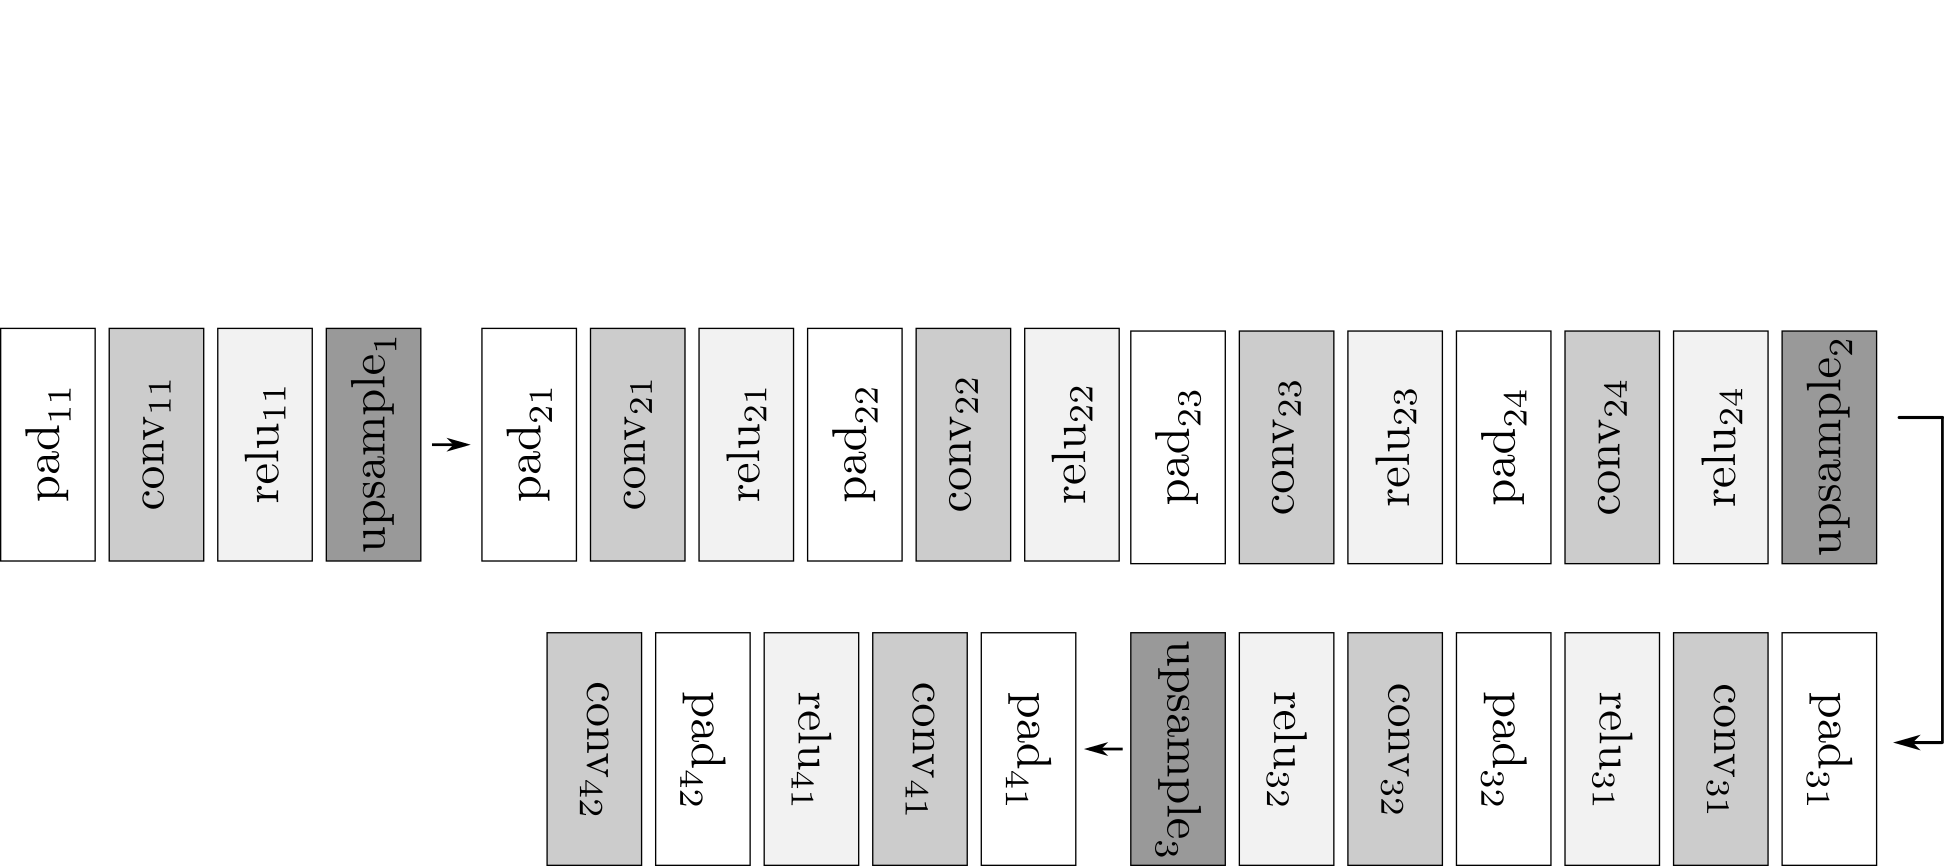
\includegraphics[width=0.75\textwidth]{Decoder_layers}
	\caption{Decoder network broken down to its layers.}
	\label{fig:decoder_network_layers}
\end{figure}

\section{Loss}
Generally, one can think of two different losses which reconstruct the input image. Let $\mathbf{x} \in \mathbb{R}^{c' \times h' \times w'}$ be the input image and $\mathbf{x}' \in \mathbb{R}^{c' \times h' \times w'}$ the output image. 

\subsection{Per-Pixel Loss}
The per-pixel loss is defined as mean squared error between the input image and the output image. Figure \ref{fig:autoencoder_loss} shows a visualization of the loss.
\begin{align}
\mathcal{L}_{\mathrm{pp}} 
\left(
\mathbf{x},
\mathbf{x}'
\right)
= 
\frac
{1}
{c' \cdot h' \cdot w'}
\cdot 
\sum_{i=1}^{c'}
\sum_{j=1}^{h'} 
\sum_{k=1}^{w'} 
\left( 
\mathbf{x}_{ijk} 
- 
\mathbf{x}'_{ijk}
\right)
^2
\end{align}
The loss forces the pixel values of $\mathbf{x}'$ to resemble the ones of $\mathbf{x}$.

\subsection{Feature Loss}
The feature loss measures the difference between the feature maps of the input image and the feature maps of the output image. It is defined as perceptual loss in the encoder network. Figure \ref{fig:autoencoder_loss} shows a visualization of the loss.
\begin{align}
\mathcal{L}_{\mathrm{feat}} 
\left(
\mathbf{F}^{(\mathbf{x})}_{ij}, 
\mathbf{F}^{(\mathbf{x}')}_{ij}
\right)
= 
\frac
{1}
{c \cdot h \cdot w} 
\cdot
\sum_{i=1}^{c} 
\sum_{j=1}^{h \cdot w} 
\left( 
\mathbf{F}^{(\mathbf{x})}_{ij} 
- 
\mathbf{F}^{(\mathbf{x}')}_{ij}
\right)
^2
\end{align}
The similarity between images in the feature space of a high performing CNN correlates well with the human perceptual similarity \cite{LPIPS_2018_CVPR}. By matching the feature maps of the input image, the output image is urged to be perceptually similar to the input image.
% figure
\begin{figure}[!ht]
	\centering
  	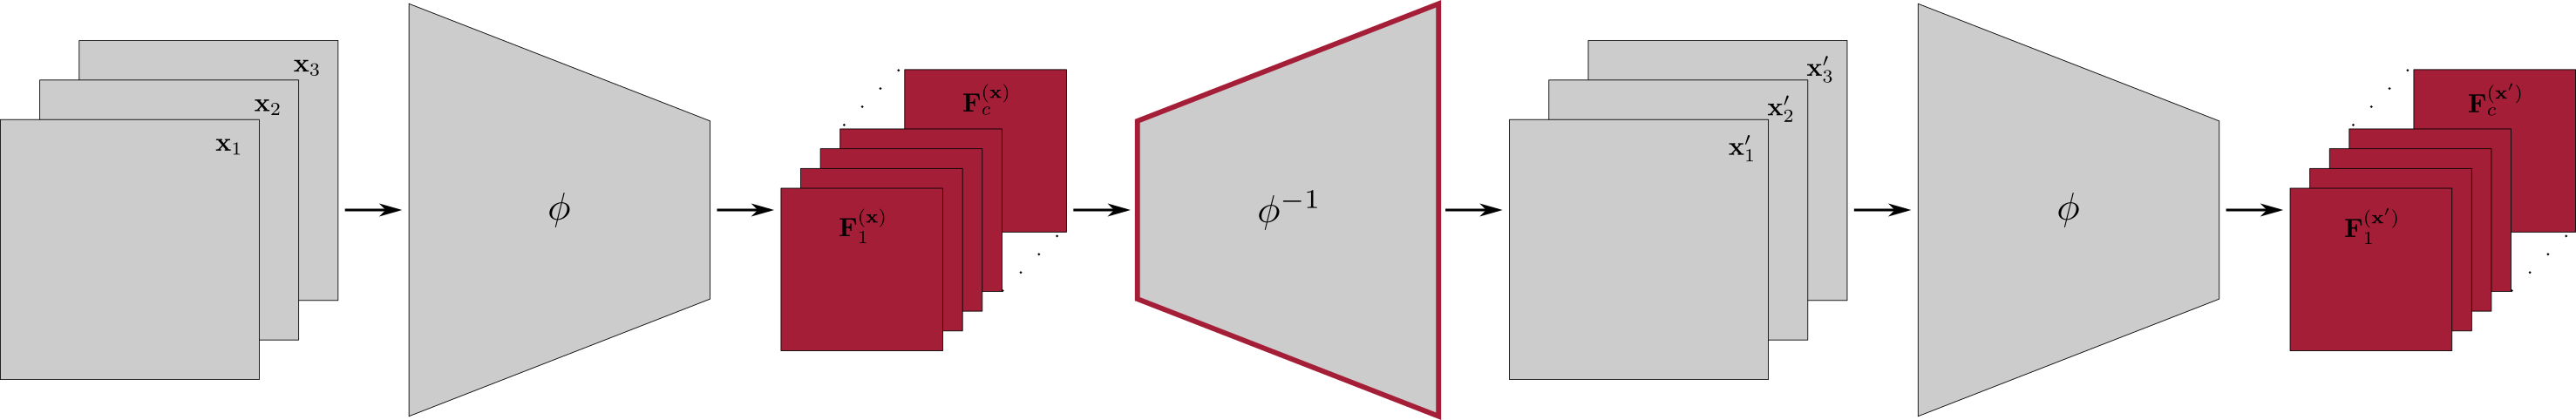
\includegraphics[width=\textwidth]{EncoderDecoder_feat}
  	\vspace{2em}
	\hdashrule{\textwidth}{0.4pt}{3mm}
	\vspace{3em}
  	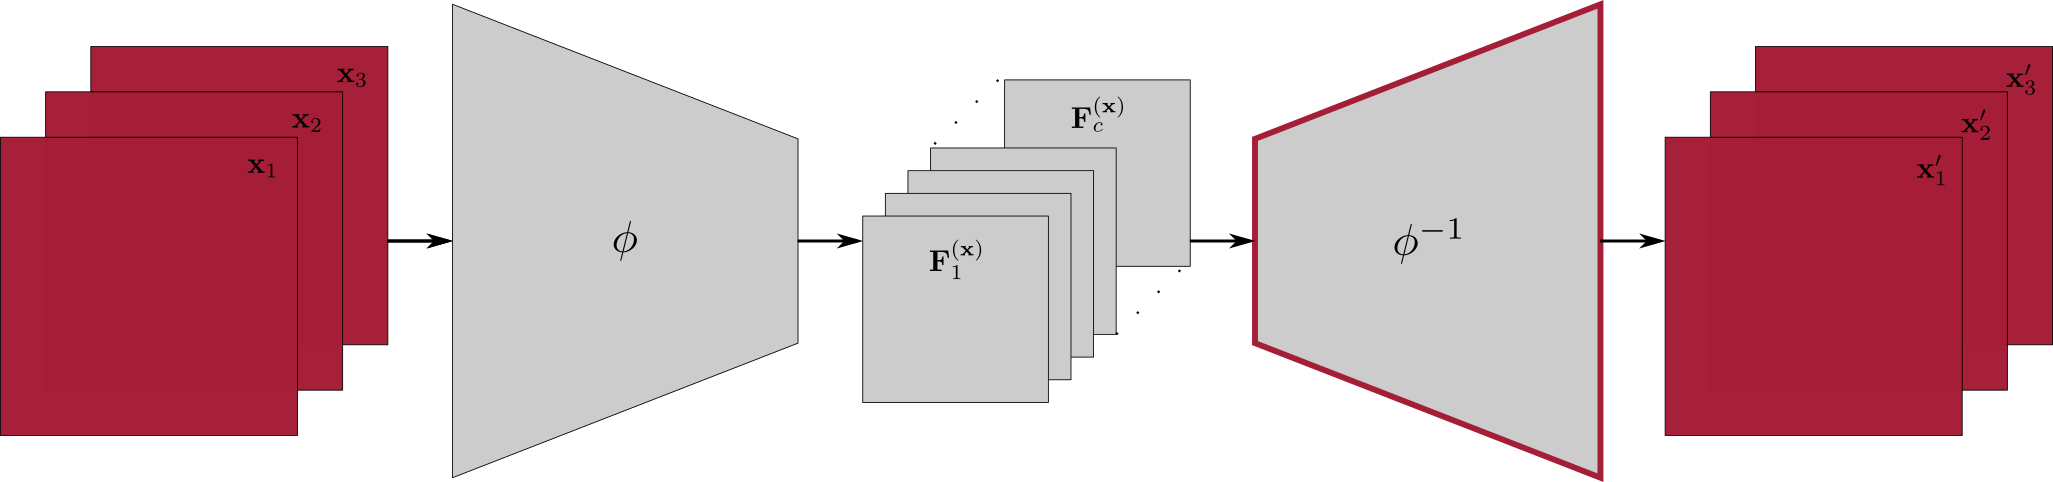
\includegraphics[width=0.65\textwidth]{EncoderDecoder_pp}
	\caption{Loss visualization of feature loss (above the dashed line) and per-pixel loss (below the dashed line) in the autoencoder network. Parts that are colored red represent where the loss is computed on. Bordered red parts represent which weights are changed by gradient descent.}
	\label{fig:autoencoder_loss}
\end{figure}

\subsection{Total Variational Regularizer}
A Total Variational (TV) regularizer penalizes high frequency structures in the input image by minimizing the sum of derivatives of the image in $h'$ and $w'$ direction. The TV loss thereby reduces checkerboard artifacts. Also, it smoothens the image especially edges and regular structures.
\begin{align}
\mathcal{L}_{\mathrm{TV}} 
\left(
\mathbf{x}'
\right)
= 
\frac
{1}
{c'} 
\cdot
\sum_{i=1}^{c'} 
\left(
\left|
\frac
{\partial \mathbf{x}_i'}
{\partial h'}
\right|
+
\left|
\frac
{\partial \mathbf{x}_i'}
{\partial w'}
\right|
\right)
^2
\end{align}

The total loss is a weighted sum of the presented losses and can be written as follows.
\begin{align}\label{eq:autoencoder_loss_total}
\mathcal{L}
= 
\lambda_{\mathrm{pp}}
\cdot
\mathcal{L}_{\mathrm{pp}} +
\lambda_{\mathrm{feat}}
\cdot
\mathcal{L}_{\mathrm{feat}} +
\lambda_{\mathrm{TV}}
\cdot
\mathcal{L}_{\mathrm{TV}}
\end{align}

\section{Training}
Since the decoder has to revert content images that are rendered in a certain style from the feature space to the image space, it is trained on a content image dataset as well as on a style image dataset.

Content images are taken from the MS-COCO dataset \cite{Lin_2014_ECCV} and style images are taken from the Kaggle painter-by-numbers competition \cite{kaggle_painter_by_numbers}. Each dataset contains about $80, 000$ images.

The autoencoder is trained for $200$ epochs. The Adam optimizer \cite{Adam_2015_ICLR} is used with a learning rate of $10^{-4}$ and $\beta_1 = 0.9, \beta_2 = 0.999$.

\section{Experiments}
The best results are achieved by balancing the three loss terms as follows.
\begin{align}
\lambda_{\mathrm{pp}} = 25, \quad \lambda_{\mathrm{feat}} =1, \quad \lambda_{\mathrm{TV}} = 10^{-6}
\end{align}
An ablation study exploring the balancing problem can be found in Appendix \ref{A:sec:balancing_of_feature_loss_and_per_pixel_loss}. Figure \ref{fig:autoencoder_images} shows some content images and style images produced by the autoencoder and the ground truth.
% figure
\begin{figure}[!ht]
\minipage{0.5\textwidth}
  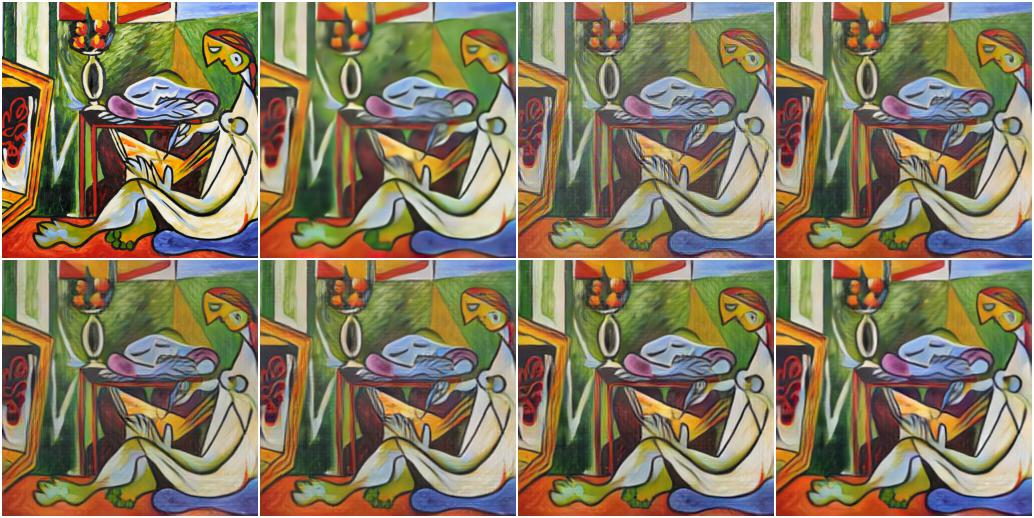
\includegraphics[width=\linewidth]{img/EncoderDecoder/A.jpeg}
\endminipage\hfill
\minipage{0.5\textwidth}
  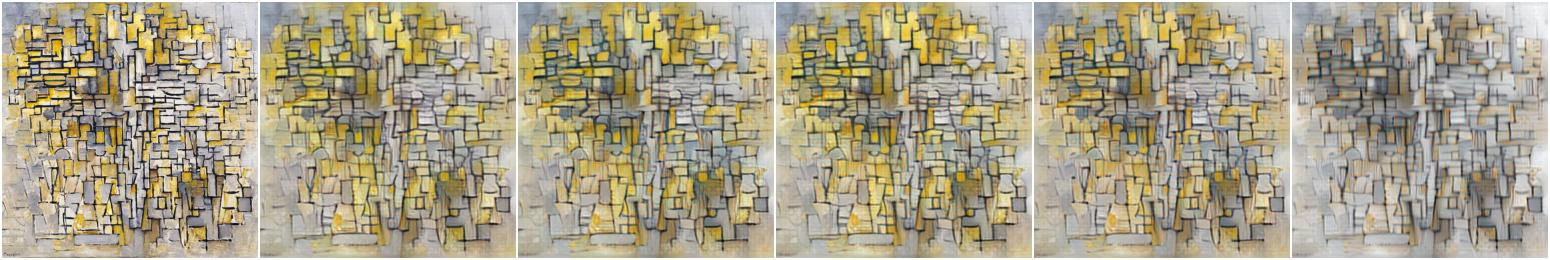
\includegraphics[width=\linewidth]{img/EncoderDecoder/B.jpeg}
\endminipage\hfill
\minipage{0.5\textwidth}
  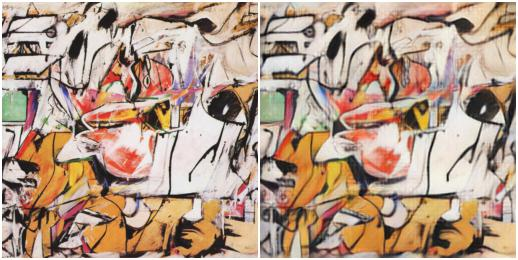
\includegraphics[width=\linewidth]{img/EncoderDecoder/C.jpeg}
\endminipage\hfill
\minipage{0.5\textwidth}
  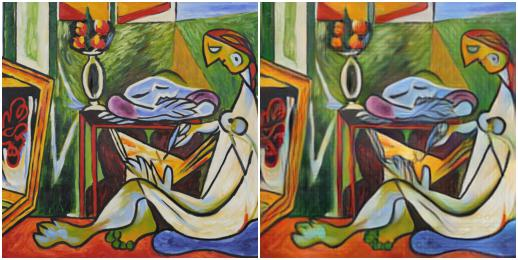
\includegraphics[width=\linewidth]{img/EncoderDecoder/D.jpeg}
\endminipage\hfill
\minipage{0.5\textwidth}
  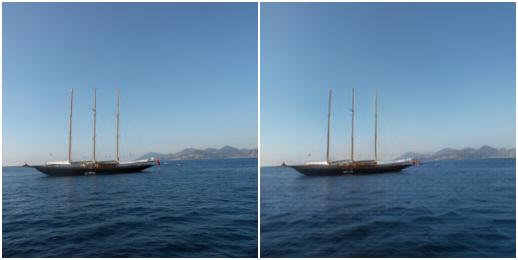
\includegraphics[width=\linewidth]{img/EncoderDecoder/E.jpeg}
\endminipage\hfill
\minipage{0.5\textwidth}
  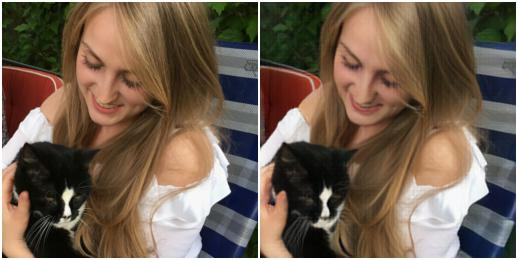
\includegraphics[width=\linewidth]{img/EncoderDecoder/F.jpeg}
\endminipage\hfill
  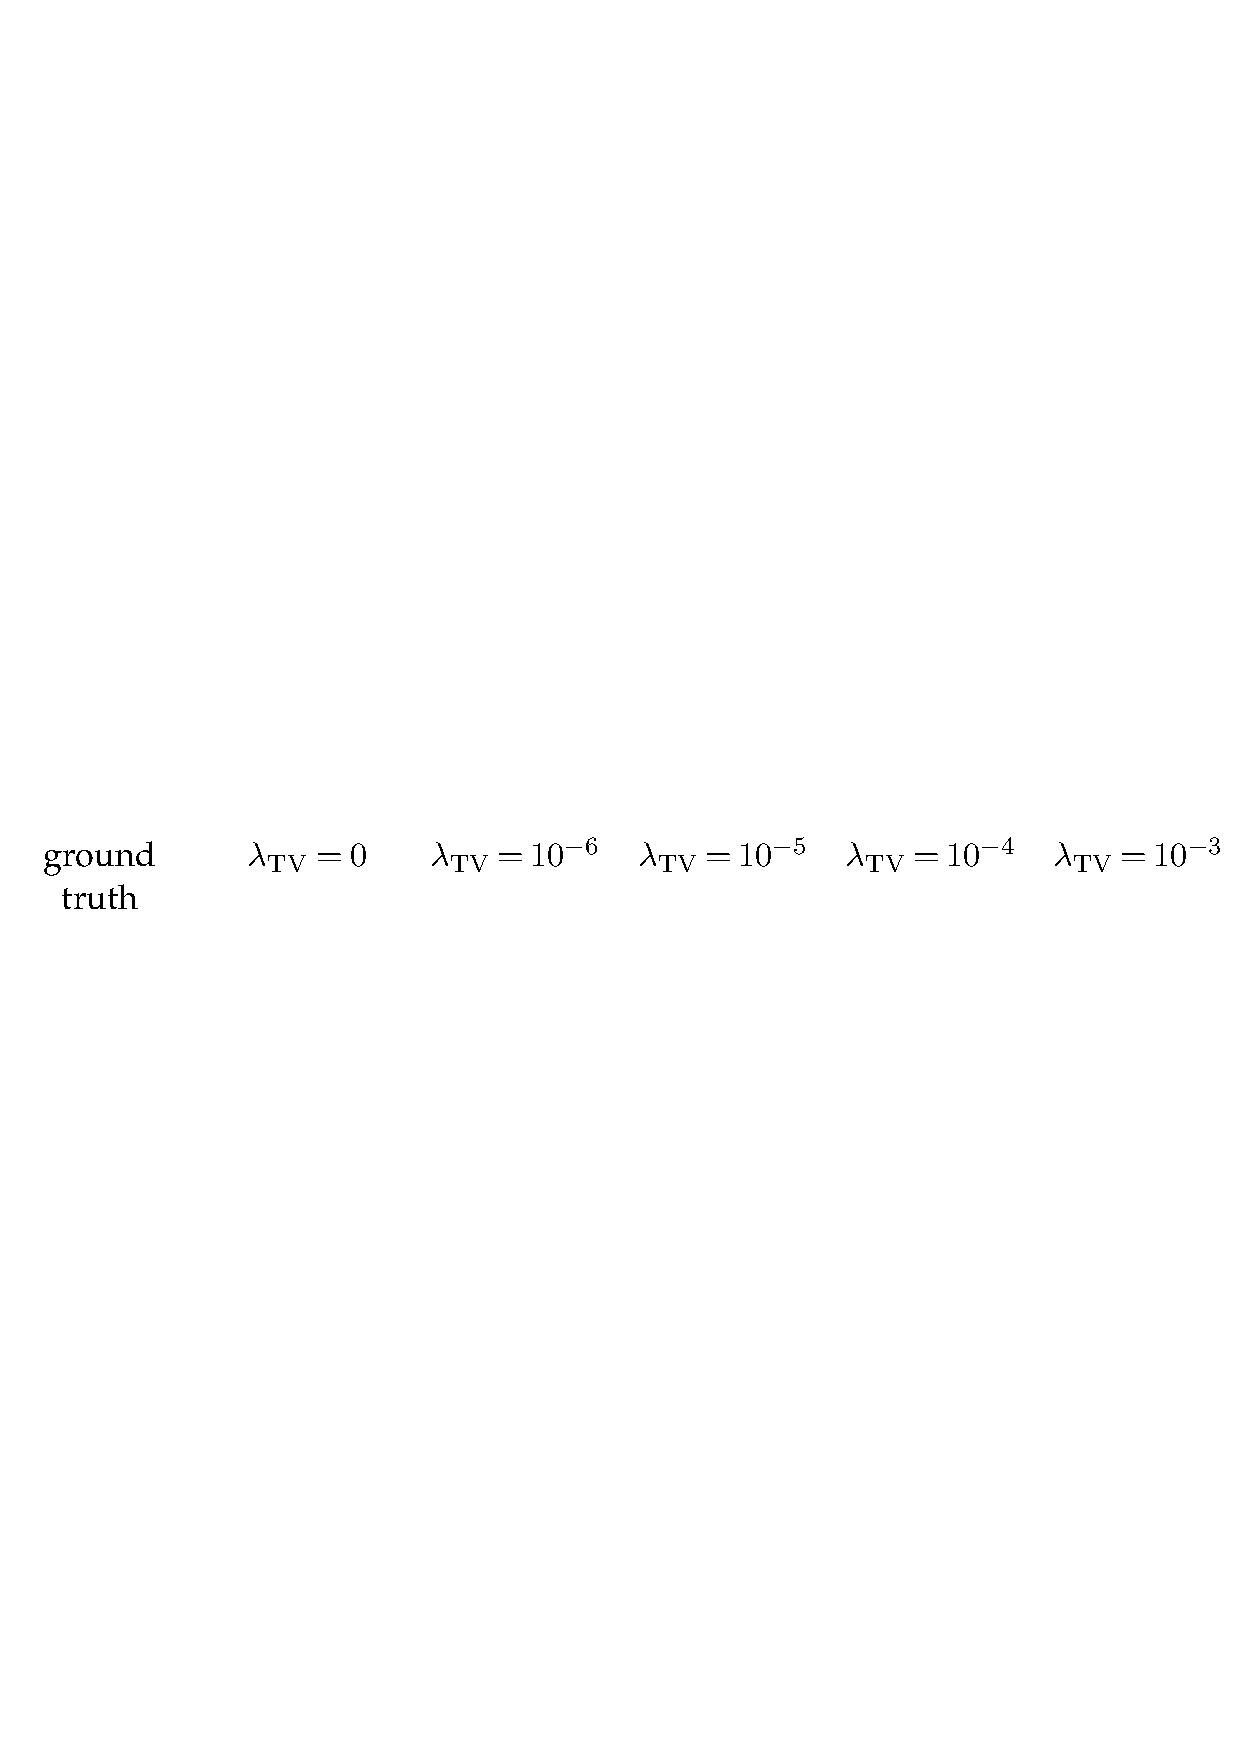
\includegraphics[width=\linewidth]{img/EncoderDecoder/ann.pdf}
  \caption{Image examples produced by the autoencoder.}
  \label{fig:autoencoder_images}
\end{figure}